\section{作品概述}

\subsection{功能与特性}

本作品面向桌面紧固件分拣，将中文任务输入、双相机感知和机械臂执行接入同一控制台（图~\ref{fig:overview}），主要功能如下：

\begin{itemize}
  \item \textbf{中文任务输入}：支持指定类别、数量和目标托盘，例如“把所有小螺母放到左盘”。规则优先解析常用指令，本地大模型处理规则无法解析的表达，校验后生成结构化任务描述。
  \item \textbf{四类零件识别与定位}：头部 RGB-D 相机识别 M12 螺丝、M12 螺母、M6 螺丝和 M6 螺母，结合深度与标定参数计算基座坐标和抓取方向。
  \item \textbf{抓取前视觉纠偏}：机械臂接近目标后，腕部相机测量局部偏差，系统修正夹爪位置后下降夹取。
  \item \textbf{执行后核对与复审}：头部相机逐槽核对放置结果，本地视觉语言模型结合前后画面生成中文复审说明。
  \item \textbf{拖动示教与数字孪生}：重力补偿辅助人工拖动，支持记录关节姿态和运动轨迹，三维模型随实测关节状态更新。
  \item \textbf{硬件执行保护}：PL 检查控制租约、反馈时效、设定范围和持续跟踪误差，按对应条件触发保护。
\end{itemize}

\begin{figure}[H]
  \centering
  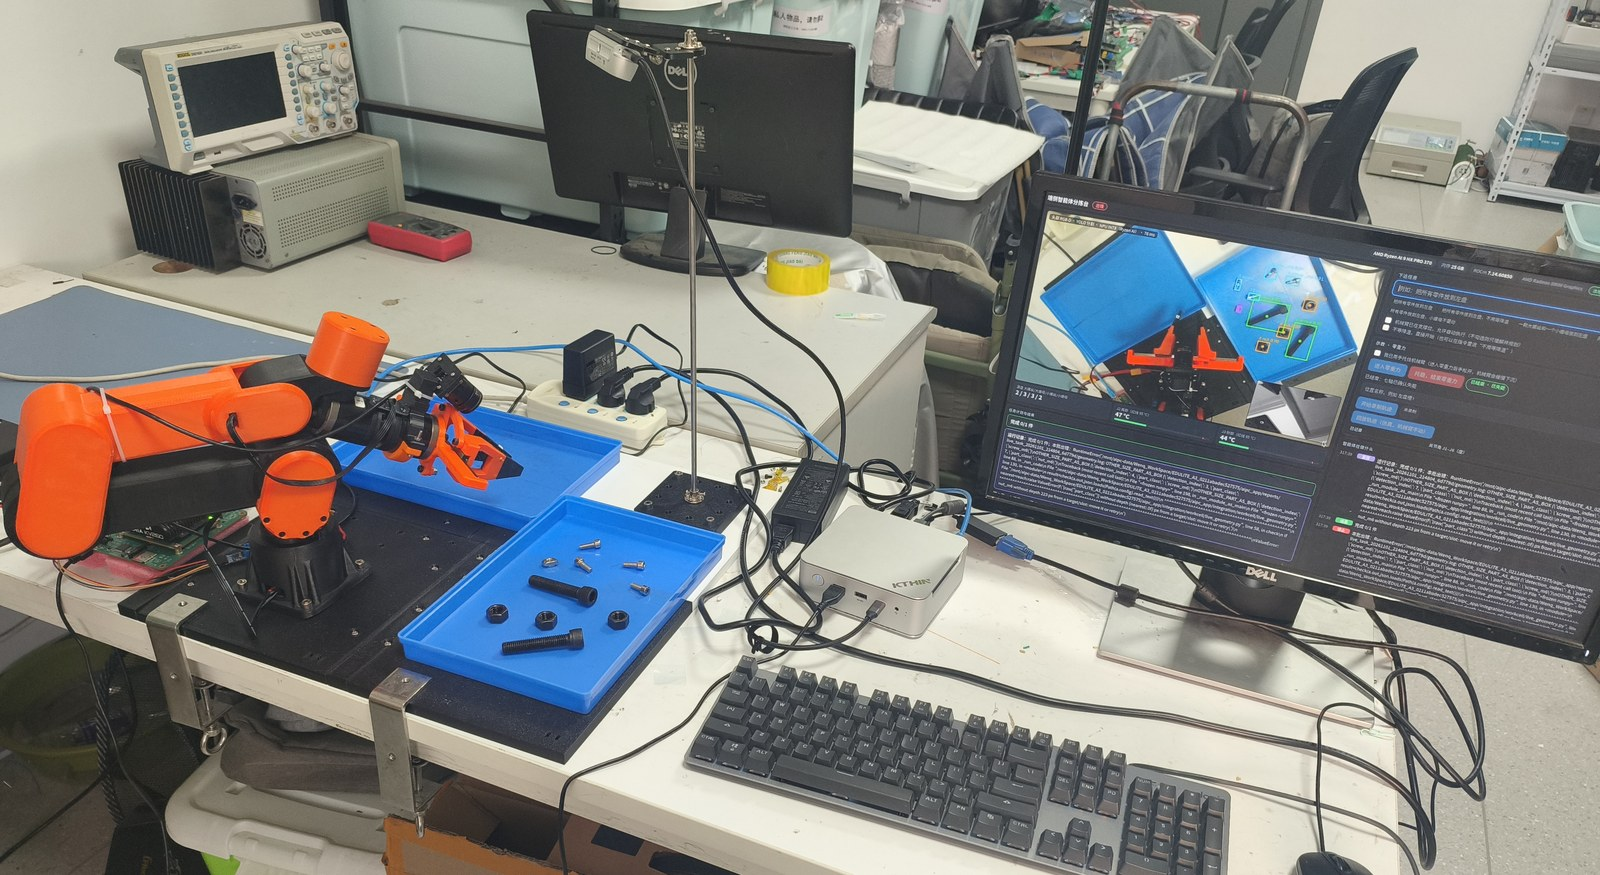
\includegraphics[width=.95\linewidth]{system_overview.jpg}
  \caption{作品全景（斜 45°）：机械臂、左右托盘、头部相机、AI PC 与上位机控制台}\label{fig:overview}
\end{figure}

\subsection{应用领域}

作品以装配配料、维修备件整理中的紧固件分拣为应用背景。用户通过中文指令调整分拣类别和数量，例如从混合零件中挑出小螺母，或将指定数量的螺丝补到目标盘。这种交互方式适合小批量、多任务的桌面工位。

系统采用本地推理，感知、规划和执行模块可分别扩展，也适合作为具身智能、嵌入式控制与 FPGA 教学实验平台。新增零件时可补充训练样本和抓取参数；调整工位时可利用拖动示教记录，为点位配置提供参考。

\subsection{主要技术特点}

\begin{enumerate}
  \item \textbf{NPU 与 GPU 分工}：NPU 运行常驻零件分割，GPU 运行本地大模型，减轻持续检测与大模型生成之间的计算资源竞争。
  \item \textbf{PL 承担周期执行}：已提交的轨迹由 PL 按 5\ms 周期求值并调度 CAN 发送，控制节拍由硬件计数器和截止期队列维持。
  \item \textbf{板端完成局部纠偏}：连续对准在 KV260 内计算视觉修正量，PL 限制关节偏移及其变化速度，减少控制数据的跨机往返。
  \item \textbf{任务与版本关联}：作业包通过内容摘要标识，执行前核对文件、任务和视觉回复的一致性，运行后保留执行及核验记录。
\end{enumerate}

\subsection{主要性能指标}

\begin{table}[H]
  \centering\small
  \caption{主要性能指标（测量条件与证据文件见第三部分与 \texttt{metrics/metrics.csv}）}\label{tab:kpi}
  \begin{tabularx}{\linewidth}{@{}>{\raggedright\arraybackslash}p{4.6cm} Y@{}}
    \toprule
    指标 & 实测值 \\
    \midrule
    零件分割精度 & 掩码 mAP50 0.976，mAP50-95 0.729（四类，验证 imgsz=1280） \\
    检测延迟（单帧，含全分辨率掩码） & GPU P50 45.4\ms；NPU P50 72.1\ms \\
    大模型同载下检测 P95 & NPU 120→141\ms；GPU 67→306\ms \\
    5\ms 周期间隔偏差 & P50 0.4\us，P95 67.0\us（15364 个周期，逻辑分析仪） \\
    PL 掩码核 / ARM 单核 & 7.82 / 14.43\ms，每帧 CPU 耗时降低 95\% \\
    板端对准收敛（大螺丝） & P50 1.06\,s（12/12 次收敛） \\
    视觉到修正指令延迟 & P50 123.0\ms，P95 206.0\ms（407 帧） \\
    跟踪看门狗检测延迟 & PL 300.8\ms；ARM 采样判据 408.1\ms \\
    FPGA 时序 & 100\,MHz，WNS +0.150\,ns，TNS 0.000\,ns \\
    AI PC $\leftrightarrow$ KV260 & RTT P50 0.169\ms，丢包 0.0\% \\
    开发记录中的放置确认比例 & 83/104（79.8\%，数量统计完整的记录），头部相机逐槽核对 \\
    \bottomrule
  \end{tabularx}
\end{table}

\subsection{主要创新点}

\begin{enumerate}
  \item \textbf{面向并发任务的端侧 AI 分工}：将 NPU 常驻分割与 GPU 大模型推理分开部署，用同载测试验证检测尾延迟的改善。
  \item \textbf{视觉与执行在板端衔接}：腕部连续纠偏在 KV260 内完成，由 PL 通道约束修正幅度和速度，缩短局部反馈路径。
  \item \textbf{周期控制与保护一体实现}：PL 集成轨迹求值、CAN 调度、执行保护和图像预处理，以总线实测和软硬件对照验证效果。
\end{enumerate}

\subsection{设计流程}

项目先完成 CAN 通信与轨迹执行，再建立头部识别、空间标定和抓取规划，随后接入腕部纠偏、中文任务接口与结果核验（图~\ref{fig:flow}）。各阶段通过仿真、板端测试和实物运行检查，结合逻辑分析仪、功率读数及任务日志评估表现。大模型工具辅助编码、测试与故障分析，协作记录见附录~\ref{app:collab}。

\begin{figure}[H]
\centering
\begin{tikzpicture}[
  node distance=4mm and 3mm,
  st/.style={draw=blue!60!black,fill=blue!6,rounded corners=2pt,align=center,font=\footnotesize,minimum height=10mm,text width=25mm},
  ar/.style={-{Stealth[length=2mm]},thick,blue!50!black}]
  \node[st] (a) {需求分析\\评分项拆解};
  \node[st,right=of a] (b) {执行层\\CAN · 轨迹 · 守护};
  \node[st,right=of b] (c) {感知层\\采集 · 训练 · 量化};
  \node[st,right=of c] (d) {两端协同\\作业包 · 板端闭环};
  \node[st,below=of d] (e) {实测迭代\\逻辑分析仪 · 功率};
  \node[st,left=of e] (f) {功能扩展\\纠偏 · 复审 · 示教};
  \node[st,left=of f] (g) {归档与复用\\技能包 · 文档};
  \draw[ar] (a)--(b); \draw[ar] (b)--(c); \draw[ar] (c)--(d); \draw[ar] (d)--(e); \draw[ar] (e)--(f); \draw[ar] (f)--(g);
  \begin{scope}[on background layer]
    \node[draw=orange!70!black,fill=orange!8,rounded corners=2pt,fit=(a)(d)(e)(g),inner sep=2.5mm] (llm) {};
  \end{scope}
\end{tikzpicture}
\caption{设计流程}\label{fig:flow}
\end{figure}
